\begin{multicols}{3}[\section{2G - GSM}]

\rhead{Autor: Kevin Taylor}
\lfoot{Letzte Bearbeitung: 16.04.2016}
\newrefsegment

\begin{boxedminipage}{\linewidth}
\begin{tabular}{p{2,1 cm}p{2.7 cm}}
\textbf{Steckbrief}& \\
\end{tabular}
\begin{tabular}{p{2,1 cm}|p{2.7 cm}}
      Einsatz seit & 1991\\
      \hline
      Frequenz"-bereich  & 900/1800/\SI{1900}{\mega\hertz}\\
      \hline
      Datenrate & \SI{9,6}{kbit/s}, \SI{14,6}{kbit/s} (brutto) \\
      \hline
      Verbreitung & Weltweit\\
      \hline
      Reichweite & \SI{35}{\kilo\metre} (ideal)\\
\end{tabular}
\end{boxedminipage}
\par
\subsection*{Überblick}
2G (engl. Abk. für second-generation) ist der Name für die zweite Generation der zellulären Telekommunikationstechnologie, die auf dem Global System for Mobile Communication Standard basiert. 
GSM wurde mit dem den folgenden Zielen versucht zu entwickeln: 
\begin{itemize}
	\item Gute Sprachqualität
	\item Günstig \& Mobil
	\item International Verfügbarkeit
	\item Effiziente Spektrumsnutzung
\end{itemize}
Zusätzlich wurden GSM Übertragungen digital verschlüsselt, sodass nur der ausgewählte Empfänger die Nachricht erhalten kann. Außerdem bot GSM neben der Telefonie auch noch andere Dienste an. Der Short-Message-Service, kurz SMS, der sich extrem hoher Beliebtheit erfreute, sowie der erste Datendienst mit einer Datenrate von bis zu 14.6 kbps.
Neben 2G GSM Standard existieren einige weniger verbreitete 2G Standards wie Nord-Amerikas IS-95 oder Japans PDC.
\cite{G2.1}
\subsection*{Technische Erläuterungen}
\subsubsection*{Grundlegende Technik}
Daten werden bei GSM mit einer Mischung von Frequenz- (FDMA - Frequency Division Multiplex Access) und Zeitmultiplexing (TDMA - Time Division Multiplex Access) übertragen. Downlink(Empfangsrichtung) und Uplink(Senderichtung) werden auf verschiedene Frequenzen durch das schon erwähnte Frequenzmultiplexing (Up=890-915Mhz, Down=935-960Mhz) aufgeteilt, diese bestehen jeweils aus 124 Kanälen a 200kHz. Die Daten selbst werden über Zeitmultiplexing versendet und empfangen. Die Rahmenzeit des Zeitmultiplexings beträgt 4,6 ms und wird in acht Zeitschlitze aufgeteilt. In einem diesem dann 0,58 ms langen „Burst“ kann nach Abzug von einer Schutzzeit 148 Bits übertragen werden.

\begin{Figure}
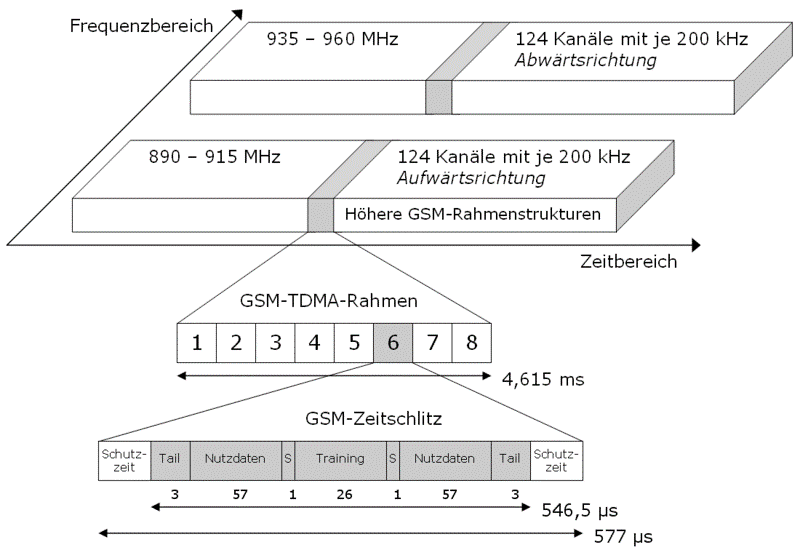
\includegraphics[width=\linewidth]{Kapitel/G2/Grafiken/GSM-Frequenzaufteilung.png}
\captionof{figure}{GSM Frequenzaufteilung~\cite{G2.3}}
\label{fig:G2.frequenzaufteilung}
\end{Figure}
\noindent
Um nun Authentifizierung, Authorisierung und eine korrekte Übertragung zu gewährleisten werden weitere Bits abgezogen, sodass am Ende eine Datenrate von 9,6 kbit/s erreicht wird. \cite{G2.1}\cite{G2.3}

\subsubsection*{Struktur des Mobilfunknetzes}
Aus der vorhergehenden Strukturerklärung sieht man, dass mit einem solchen System rund 1000 Mobilfunkgeräte gleichzeitig genutzt werden können. Dies ist für ein Globales Netz aber bei weitem nicht ausreichend. Deswegen kommt nun der zelluläre Aufbau des Netzes zum Tragen, also  die Technik des Raum-Multiplexing (SDMA - Space Division Multiplex Access).\cite{G2.2}

\begin{Figure}
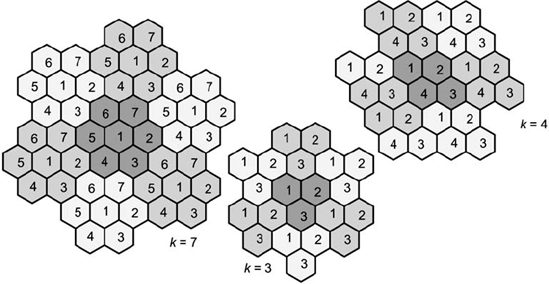
\includegraphics[width=\linewidth]{Kapitel/G2/Grafiken/GSM-Funkzellenideal.png}
\captionof{figure}{GSM Funkzellenideal~\cite{G2.2}}
\label{fig:G2.funkzellenideal}
\end{Figure}
%,height=2.5cm
Der Up- und Downlink wird hierbei nochmal in mehrere Bereiche unterteilt um Interferenzen der unterschiedlichen Netze für das SDMA zu minimieren. Diese Bereiche haben nun immer einen anderen Frequenzbereich neben sich. Dies wird vereinfacht dargestellt mit hexagonalen Waben, siehe Abbildung \ref{fig:G2.funkzellenideal}. Dies ist natürlich eine idealisierte Darstellung, wenn eine bessere Näherung wie in Abbildung \ref{fig:G2.funkzellen} aussieht, die insbesondere in städtischem Umfeld durch Häuser, Straßen, Flüsse und anderes beeinflusst wird. \cite{G2.2}

\begin{Figure}
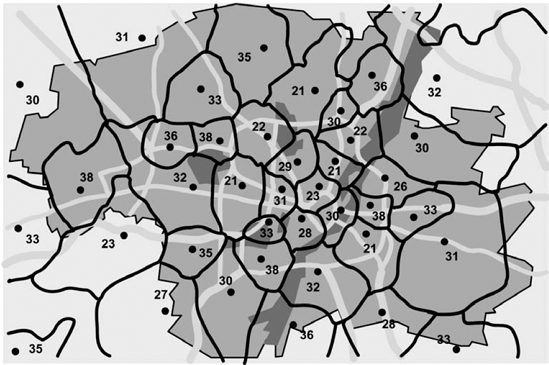
\includegraphics[width=\linewidth]{Kapitel/G2/Grafiken/GSM-Funkzellen.png}
\captionof{figure}{GSM Funkzellen~\cite{G2.2}}
\label{fig:G2.funkzellen}
\end{Figure}

Es folgt die nächste Überlegung, dass sich mobile Geräte in verschiedenen Zellen aufhalten, oder während eines laufenden Gesprächs von Zelle zu Zelle bewegen. Hierbei erfolgt ein sogenannter „Handshake“ (=engl.  Handschlag) oder Verbindungsübergabe, der die Übergabe eines Mobilen Gerätes von der aktuellen Funkzelle in das sich hinbewegende neue Funkzelle regelt.
Vereinfacht lässt sich dies in Abbildung \ref{fig:G2.handshake} beschreiben, hier spricht man von dem Mobilfunkteilnehmer, der sich automatisch in die, der Bewegungsrichtung befindenen Basisstation, einbucht während er in der vorherigen Basistation ausgebucht wird.\cite{G2.3}

\begin{Figure}
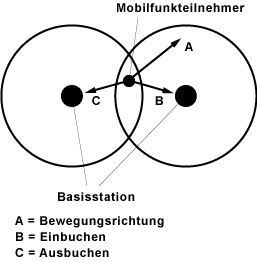
\includegraphics[width=\linewidth]{Kapitel/G2/Grafiken/GSM-Handshake.png}
\captionof{figure}{GSM Handshake~\cite{G2.2}}
\label{fig:G2.handshake}
\end{Figure}

\subsubsection*{SIM}

Das Subscriber Identiy Module, kurz SIM oder oft SIM-Card genannt, ist ein Chip den jedes GSM-Gerät beötigt um sich in ein entsprechendes Funknetz einwählen zu können. Diese SIM-Card enthät unter anderem eine International Mobile Subscriber Identity, kurz IMSI. Diese maximal 15 Zeichen lange dezimale Zahlen wird wie folgt aufgeteilt:

\begin{Figure}
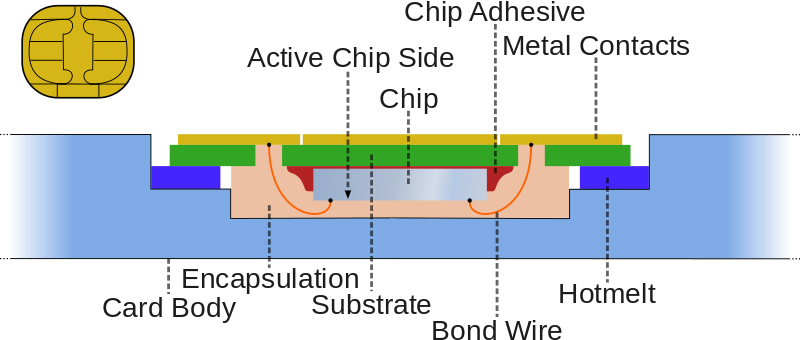
\includegraphics[width=\linewidth]{Kapitel/G2/Grafiken/GSM-SIM.png}
\captionof{figure}{GSM SIM~\cite{G2.2}}
\label{fig:G2.sim}
\end{Figure}

\begin{itemize}
	\item Mobile Country Code (MCC), drei Zahlen, International standartisiert (z.B. 262 für Deutschland)
	\item Mobile Network Code (MNC), zwei Zahlen, eindeutige Identifikation eines Netzanbieters des jeweiligen Landes (01, 02, 07 entsprechend für T-Mobile, Vodafone, O2)
	\item Mobile Subscriber Identification Number (MSIN), maximal 10 Zahlen, eindeutige Identifikation eines Nutzers in seinem Heimnetz
\end{itemize}

Nebenher bestitzt die SIM Card noch die Fähigkeiten PIN, Telefonbuch, Notizbuch, SMS und die zuletzt angerufene Telefonummer und mehr zu speichern.\cite{G2.1}

\subsubsection*{Sonstiges}

Die Leistungsaufnahme eines solchen mobilen Geräts im 900/1800Mhz Bereich liegt bei 1/2 Watt, während eine passende Basisstation 20-50/10-20 Watt je nach Empfangsdistanz benötigt.\cite{G2.2}

\subsection*{Einsatz}
Weltweit besitzt GSM 3 Milliarde Nutzer als das grundlegende mobile Kommunikationsmittel. Es ist wenn überhaupt ungewöhnlich keinen Empfang zu haben, so verbreitet ist er. (Siehe Abbildung \ref{fig:G2.global}).

%Das Bild \ref{fig:vorlage.vorlesungssaal} hat eigentlich keinen Bezug zu dem ganzen Text. Erzeugt jedoch einen ordentlichen und schönen Einblick in einen Vorlesungssaal, den man zweimal im Jahr betritt.

\end{multicols}
\newpage
\section*{Historische Entwicklung}
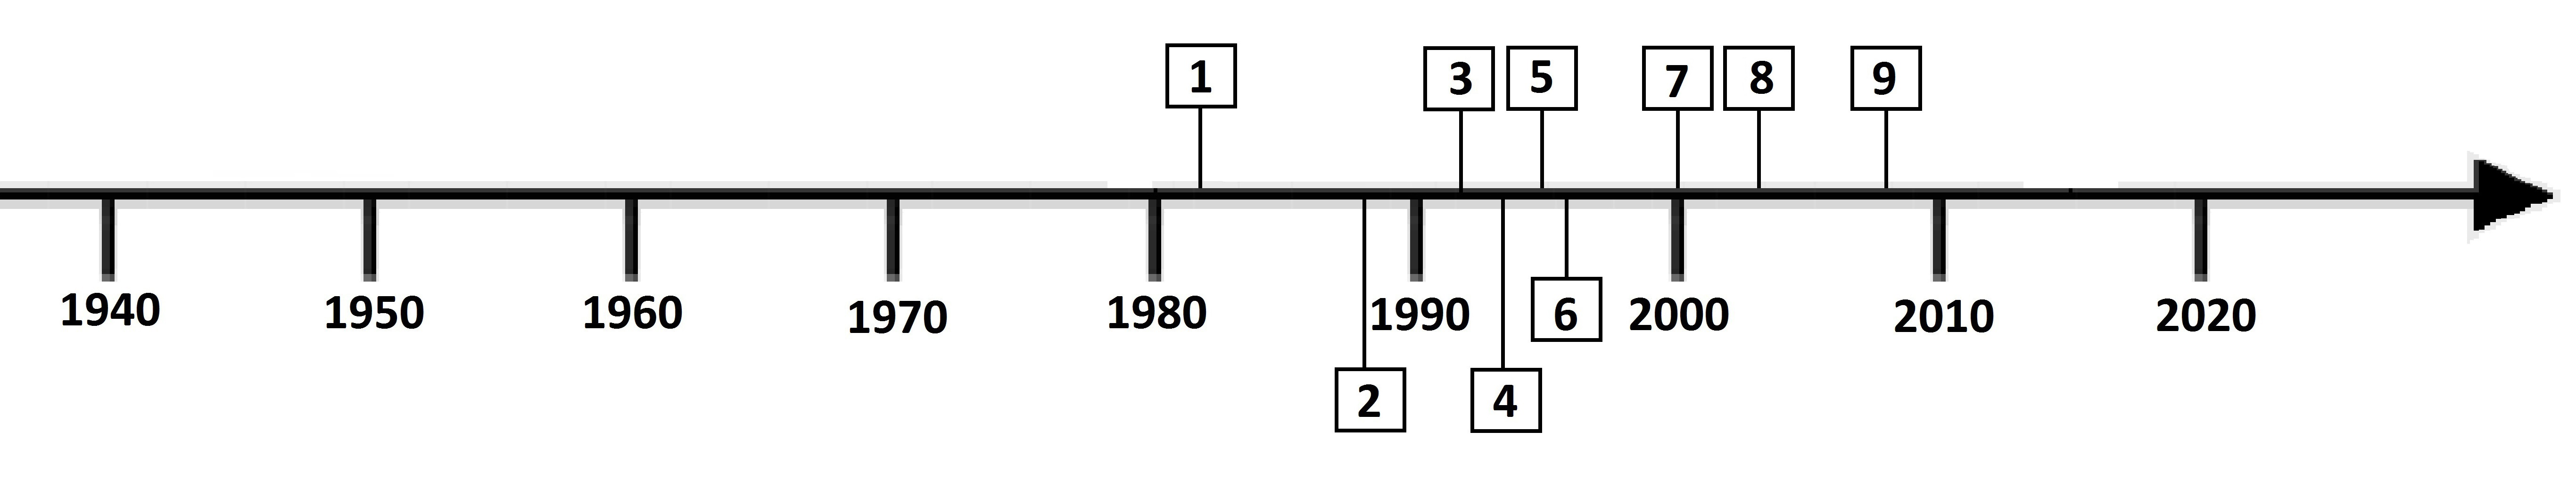
\includegraphics[width=\textwidth]{Kapitel/G2/Grafiken/Zeitstrahl}
\par
\noindent
\begin{tabular}{|p{1 cm}|p{3 cm}|p{13.55 cm}|}
	\hline
	Nummer & Datum & Entwicklungsschritte~ \cite{G2.1}\cite{G2.3}\\
	\hline
	1 & 1982 & Die Groupe Spécial Mobile wird eingerichtet und die Entwicklung an einem globalen Mobilfunkstandard, von der CEPT (European Conference of Postal and Telecommunications Administrations) beauftragt.\\
	\hline
	2 & 1986 & Die Entscheidung für das 900Mhz Spektrum für das GSM Band fällt.\\
	\hline
	3 & 1991 & Der erste GSM Anruf wurde in Finnland von Radiolinja durchgeführt und leutet somit den Beginn des GSM Mobilfunkstandards ein.\\
	\hline
	4 & 1992 & Die erste SMS wird versendet.\\
	\hline
	5 & 1993 & Das erstes GSM Mobiltelefon Nokia 1011 ist kommerziell erhätlich.\\
	\hline
	6 & 1995 & Die Dienste über GSM angeboten werden erweitern sich um Fax, Daten und SMS Dienste.\\
	\hline
	7 & 2000 & Der General Packet Radio Service, kurz GPRS, steht nun zur Verfügung.\\
	\hline
	8 & 2003 & Enhanced Data Rates for GSM Evolution, kurz EDGE, steht nun zur Verfügung.\\
	\hline
	9 & 2008 & Weltweit erfreut sich der 2G Mobilfunk mehr als drei Milliarde Nutzer.\\
	\hline
\end{tabular}
\par
\begin{multicols}{3}

\subsection*{Anbieter und Gremien}
Um ein europaweites Kommunikationsnetz zu entwicklen wurde die Groupe Spécial Mobile von der CEPT (Conférence Européenne des Administrations des Postes et des Télécommunications) ins Leben gerufen, die ab 1989 in der ETSI aufging und das heutige Backroynm für GSM (Global System for Mobile Communication) entstanden ist. Diese bietet für GSM Operatoren ein Memorandum of Understanding an(im Prinzip ein Standard), was 2008 von 747 Mitgliedern unterschrieben wurde, die 670 GSM Netze in 200 Ländern betreiben. \cite{G2.3}	

\subsection*{Ausblick}
Wie schon erwähnt lag die Nutzerzahl 2008 bei 3 Milliarden Nutzer. Trotzdem fangen erste Länder an G2 auszumustern. Macau ist hier Vorreiter, knapp gefolgt von Singapur, Australien und dem größten Mobilfunkanbieter der USA, AT\&T.
Dies würde die Frequenzbereiche für die neuere Standards befreien. Doch gibt es auch viele Netzbetreiber, insbesondere in Europa, die sich Zeit lassen werden, da mit Roaminggebühren immer noch Geld verdient werden kann.\cite{G2.3}~(Bildquelle:~\cite{G2.4})
\printbibliography[segment=6,heading=subbibliography]

\end{multicols}
\begin{Figure}
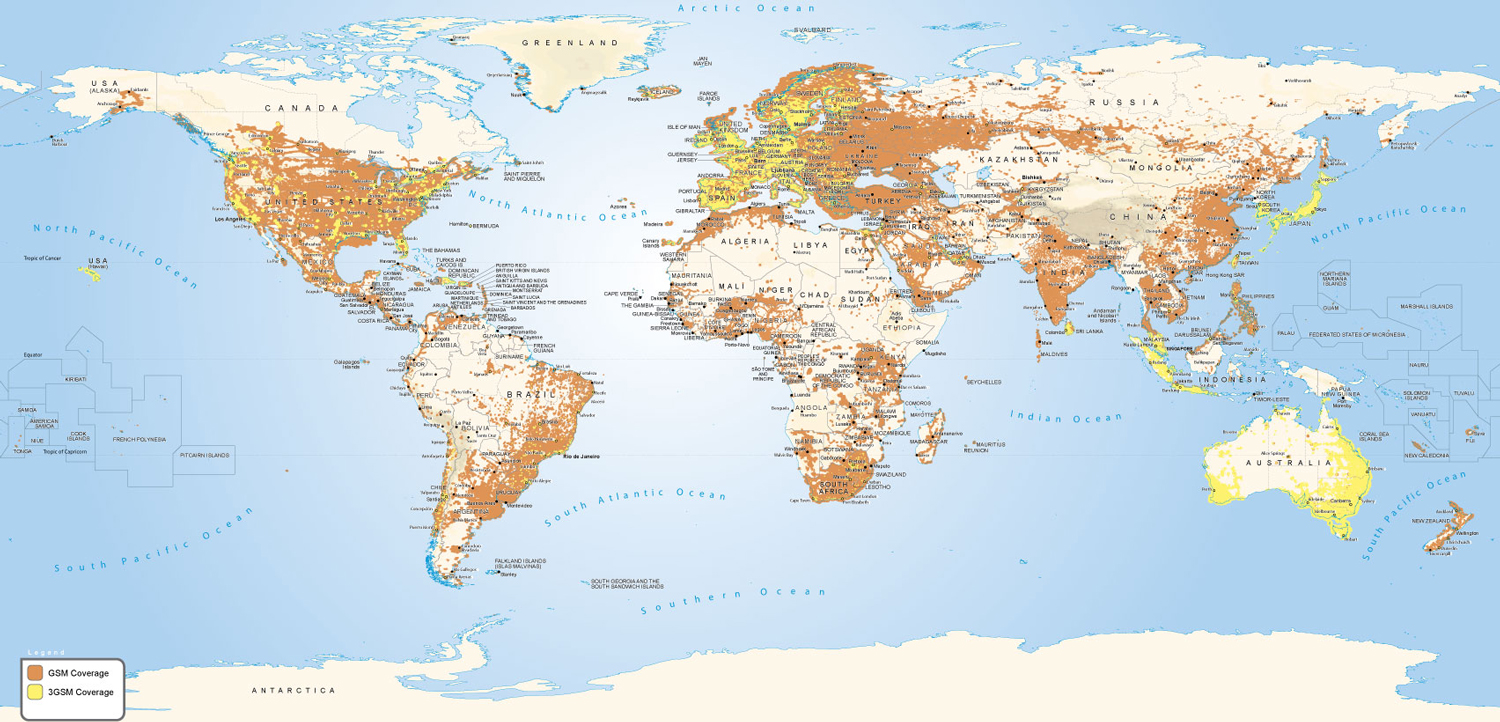
\includegraphics[width=\textwidth]{Kapitel/G2/Grafiken/GSM-Netzabdeckung-Weltweit.jpg}
\captionof{figure}{Globable Netzabdeckung (orange: GSM, gelb: UMTS)~\cite{G2.4}}
\label{fig:G2.global}
\end{Figure}
\newpage